\documentclass{article}

% if you need to pass options to natbib, use, e.g.:
% \PassOptionsToPackage{numbers, compress}{natbib}
% before loading nips_2016
%
% to avoid loading the natbib package, add option nonatbib:
% \usepackage[nonatbib]{nips_2016}

% \usepackage{nips_2016}

% to compile a camera-ready version, add the [final] option, e.g.:
\usepackage[final,nonatbib]{nips_2016}

\usepackage[utf8]{inputenc} % allow utf-8 input
\usepackage[T1]{fontenc}    % use 8-bit T1 fonts
\usepackage{hyperref}       % hyperlinks
\usepackage{url}            % simple URL typesetting
\usepackage{booktabs}       % professional-quality tables
\usepackage{amsfonts}       % blackboard math symbols
\usepackage{nicefrac}       % compact symbols for 1/2, etc.
\usepackage{microtype}      % microtypography
\usepackage{color}
\usepackage{graphicx}
\usepackage{amssymb,amsthm,amsfonts,amsmath,graphicx}    
\usepackage[shortlabels]{enumerate}
\usepackage[options ]{algorithm2e}
\graphicspath{ {../figures/} }

\newcommand{\ind}[1]{1_{#1}} % Indicator function
\newcommand{\pr}{P} % Generic probability
\newcommand{\ex}{E} % Generic expectation
\newcommand{\var}{\textrm{Var}}
\newcommand{\cov}{\textrm{Cov}}
\newcommand{\sgn}{\textrm{sgn}}
\newcommand{\sign}{\textrm{sign}}
\newcommand{\kl}{\textrm{KL}} 
\newcommand{\abs}[1]{|{#1}|}



\renewcommand{\S}{\Sigma}
\renewcommand{\L}{\Lambda}
\renewcommand{\[}{\begin{equation}}
\renewcommand{\]}{\end{equation}}
\renewcommand{\b}{\backslash}
\newcommand{\g}{\,\vert\,}
\newcommand{\tr}{\mathrm{tr}}
\newcommand{\diag}{\mathrm{diag}}
\newcommand{\bea}{\begin{eqnarray}}
\newcommand{\eea}{\end{eqnarray}}
\newcommand{\hx}{\hat{x}}
\newcommand{\hxi}{\hat{\xi}}
\newcommand{\Var}{\mathrm{Var}}
\newcommand{\Cov}{\mathrm{Cov}}
\newcommand{\prop}{\propto}
\newcommand{\deq}{:=}

\newcommand{\EE}{\mathbb{E}}
\newcommand{\II}{\mathbb{I}}
\newcommand{\R}{\mathbb{R}}
\newcommand{\PP}{\mathbb{P}}

\newcommand{\La}{\mathcal{L}}

\newcommand{\n}{\mathcal{N}}

\newcommand{\bx}{\mathbf{x}}
\newcommand{\bX}{\mathbf{X}}
\newcommand{\by}{\mathbf{y}}
\newcommand{\bs}{\mathbf{s}}
\newcommand{\bn}{\mathbf{n}}
\newcommand{\br}{\mathbf{r}}
\newcommand{\bt}{\mathbf{t}}

\newcommand{\fig}[1]{Figure~\ref{fig:#1}}
\newcommand{\chap}[1]{Chapter~\ref{chap:#1}}
\newcommand{\mysec}[1]{Section~\ref{sec:#1}}
\newcommand{\app}[1]{Appendix~\ref{sec:#1}}
\newcommand{\eq}[1]{Eq.~(\ref{eq:#1})}
\newcommand{\eqs}[1]{Eqs.~(\ref{eq:#1})}
\newcommand{\eqss}[1]{(\ref{eq:#1})}
\newcommand{\thm}[1]{Theorem~\ref{thm:#1}}

\newcommand{\indep}{{\;\bot\!\!\!\!\!\!\bot\;}}
\newcommand{\eps}{\varepsilon}

\newcommand{\one}{1}
\newcommand{\Dir}{{\rm Dir}}
\newcommand{\Mult}{{\rm Mult}}
\newcommand{\Bin}{{\rm Bin}}
\newcommand{\Ga}{{\rm Ga}}
\newcommand{\IG}{{\rm IG}}
\newcommand{\InvGa}{{\rm IG}}
\newcommand{\Chisquare}{\Chi^2}
\newcommand{\St}{{\rm St}}
\newcommand{\Beta}{{\rm Beta}}
\newcommand{\iid}{i.i.d.}
\newcommand{\Eta}{{\cal N}}
\newcommand{\Ber}{{\rm Ber}}

\newcommand{\simiid}{\stackrel{\tiny\text{iid}}{\sim}}
\newcommand{\simind}{\stackrel{\tiny\text{ind}}{\sim}}

\DeclareMathOperator*{\BP}{BP}
\DeclareMathOperator*{\DP}{DP}
\DeclareMathOperator*{\GP}{GP}
\DeclareMathOperator*{\BeP}{BeP}

% Caligraphic alphabet
\newcommand{\calr}{\mathcal{R}} % only because \cr already taken
\newcommand{\ca}{\mathcal{A}} \newcommand{\cb}{\mathcal{B}} \newcommand{\cc}{\mathcal{C}} \newcommand{\cd}{\mathcal{D}} \newcommand{\ce}{\mathcal{E}} \newcommand{\cf}{\mathcal{F}} \newcommand{\cg}{\mathcal{G}} \newcommand{\ch}{\mathcal{H}} \newcommand{\ci}{\mathcal{I}} \newcommand{\cj}{\mathcal{J}} \newcommand{\ck}{\mathcal{K}} \newcommand{\cl}{\mathcal{L}} \newcommand{\cm}{\mathcal{M}} \newcommand{\cn}{\mathcal{N}} \newcommand{\co}{\mathcal{O}} \newcommand{\cp}{\mathcal{P}} \newcommand{\cq}{\mathcal{Q}} \newcommand{\cs}{\mathcal{S}} \newcommand{\ct}{\mathcal{T}} \newcommand{\cu}{\mathcal{U}} \newcommand{\cv}{\mathcal{V}} \newcommand{\cw}{\mathcal{W}} \newcommand{\cx}{\mathcal{X}} \newcommand{\cy}{\mathcal{Y}} \newcommand{\cz}{\mathcal{Z}}

% Convergence
\newcommand{\convd}{\stackrel{d}{\longrightarrow}} % convergence in distribution/law/measure
\newcommand{\convp}{\stackrel{P}{\longrightarrow}} % convergence in probability
\newcommand{\convas}{\stackrel{\textrm{a.s.}}{\longrightarrow}} % convergence almost surely
\newcommand{\convr}{\stackrel{r}{\longrightarrow}} % convergence in r^{th} mean

\newcommand{\eqd}{\stackrel{d}{=}} % equal in distribution/law/measure
\newcommand{\argmax}{\mathop{\mathrm{argmax}}}
\newcommand{\argmin}{\mathop{\mathrm{argmin}}}
\newcommand{\conv}{\textrm{conv}} % for denoting the convex hull


\makeatletter
\providecommand*{\diff}%
	{\@ifnextchar^{\DIfF}{\DIfF^{}}}
\def\DIfF^#1{%
	\mathop{\mathrm{\mathstrut d}}%
		\nolimits^{#1}\gobblespace}
\def\gobblespace{%
	\futurelet\diffarg\opspace}
\def\opspace{%
	\let\DiffSpace\!%
	\ifx\diffarg(%
		\let\DiffSpace\relax
	\else
		\ifx\diffarg[%
			\let\DiffSpace\relax
	\else
		\ifx\diffarg\{%
			\let\DiffSpace\relax
		\fi\fi\fi\DiffSpace}


\providecommand*{\deriv}[3][]{\frac{\diff^{#1}#2}{\diff #3^{#1}}}
\providecommand*{\pderiv}[3][]{\frac{\partial^{#1}#2}{\partial #3^{#1}}}
		
\newcommand{\threequals}{\equiv}

\usepackage{subcaption}
\renewcommand{\qedsymbol}{$\spadesuit$}

\title{Data Augmentation to Accelerate Convergence of Variational Bayes}

% The \author macro works with any number of authors. There are two
% commands used to separate the names and addresses of multiple
% authors: \And and \AND.
%
% Using \And between authors leaves it to LaTeX to determine where to
% break the lines. Using \AND forces a line break at that point. So,
% if LaTeX puts 3 of 4 authors names on the first line, and the last
% on the second line, try using \AND instead of \And before the third
% author name.

\author{
  Runjing Liu and Jake Soloff \\
  Department of Statistics, UC Berkeley\\
  \texttt{\{runjing\_liu,jake\_soloff\}@berkeley.edu}
  %% examples of more authors
  %% \texttt{email} \\
  %% \And
  %% Coauthor \\
  %% Affiliation \\
  %% Address \\
  %% \texttt{email} \\
  %% \And
  %% Coauthor \\
  %% Affiliation \\
  %% Address \\
  %% \texttt{email} \\
}

\begin{document}
% \nipsfinalcopy is no longer used

\maketitle

\vspace{-1em}

\begin{abstract}
one line\\two lines\\3 linez\\ 4 linsu
\end{abstract}

\section{Motivation}
\label{motivation}
%Voting records of legislators are commonly analyzed by political scientists to examine relationships between legislator political leanings, institutional structures, and legislative outcomes \cite{Clinton2004}. For example, even simple dimensionality reduction techniques on voting data in the US House of Representatives uncover the political characteristics of individual legislators such as party affiliation (Figure \ref{fig:DimRedux}). \par

\subsection{Optimization as Approximate Inference} 

Bayesian statistics offers a simple formula for learning from data: specify a joint distribution $p(X,\theta) = p(X\mid \theta)\,p(\theta)$ over observations $X$ and latent variables $\theta$, and quantify the uncertainty in $\theta$ conditional on seeing $X$ through the posterior distribution $p(\theta\mid X)$. In complex models, exact computation with the full posterior is intractable \cite{Cooper}; in practice, we turn to methods for approximation such as sampling (MCMC) or variational inference.

{\sl Variational Bayes} casts posterior inference as an optimization problem
\begin{align}
\min_{q}D(q(\theta)\,\|\, p(\theta\mid X)).
\end{align}
Since the KL-divergence is non-negative and vanishes precisely at $q(\theta) = p(\theta\mid X)$, this program recovers the target. We focus on variational Bayes under the na\"ive mean field assumption, which restricts the minimization in equation (1) to all distributions $q(\theta) = \prod_{i=1}^Kq(\theta_i)$ which factorize over the latent variables $\theta = \{\theta_i\}_{i=1}^K$. Noting that
\begin{align}
\mathcal L(q) :=  \mathbb E_q\left[\log\frac{p(X,\theta)}{q(\theta)}\right] =\log p(X) -  D(q(\theta)\,\|\, p(\theta\mid X)) \le \log p(X).
\end{align}
The quantity $\mathcal L(q)$ (called the ELBO) lower bounds the model evidence, and the program (1) is equivalent to maximizing $\mathcal L(q)$. We may impose parametric assumptions on each variational factor $q(\theta_i) = q_{\widehat\tau_i}(\theta_i)$ to simplify the expectations in equation (2) and optimize over the choice of $\widehat\tau_i$---though we emphasize that in many cases these additional assumptions are unnecessary \cite{Beal,Blei}. Coordinate ascent variational inference (CAVI) maximizes $\mathcal L(q)$ over each factor individually with the others held fixed. 

Note that CAVI does not recover the true posterior, in contrast with Gibbs sampling, which is {\sl asymptotically} exact. Compared to sampling, however, Variational Bayes tends to be more efficient, as we can leverage many tools from optimization. Both methods are known to converge slowly when the latent variables are well correlated in the posterior. In the appendix, we show this for a Gaussian posterior, where the rates for the Gibbs sampler (as computed in \cite{Sahu}) and CAVI actually match:

{\bf Proposition 1.} Consider a model in which the posterior distribution has form
\begin{align}
p(\theta\mid X) \triangleq \mathcal N(\mu^*,\Lambda^{-1}),
\end{align}
where $\mu^* = (\mu_1^*,\mu_2^*)^{\mathsf T}$ and $\Lambda$ has blocks $\Lambda_{11}, \Lambda_{12},$ and $\Lambda_{22}$, and these means and precisions depend implicitly on the observation $X$. Then CAVI, which updates blocks $\theta_1$ and $\theta_2$ alternatingly, converges linearly at the same rate as the corresponding Gibbs sampler.

\newpage

\subsection{Reparametrization and Data Augmentation} 

Observing the high-level connections between convergence rates for Gibbs sampling and CAVI, we posit that schemes for accelerating convergence of samplers may be successfully imported into quickly converging variational Bayesian methods, and their properties may be better understood from an optimization perspective. In particular, an important tool in the MCMC literature for reducing posterior dependencies is {\sl data augmentation}, i.e. introducing intermediate latent variables $\mu$, and calculating the posterior of $(\mu,\theta)$ given $X$. In a sampler, this requires draws from the complete conditionals $\theta_i \mid \theta_{\setminus i},\mu,X$ (or $\theta\mid \mu,X$ if possible) and $\mu \mid \theta,X$. It turns out the convergence of such a sampler depends critically on the parametrization of $\mu$. One may look to strategies for determining an appropriate parametrization \cite{Papaspiliopoulos}. 


Instead of settling on a single model for their sampler, Yu \& Meng \cite{Yu} study situations with two competing data augmentations: one in which an auxiliary variable $\mu$ is sufficient for $\theta$ (that is, $X\perp\theta\mid \mu$) and one in which an auxiliary variable $\nu$ is ancillary for $\theta$ (that is $\theta\perp \nu$). If Gibbs sampling is feasible in one model, it will likely also be feasible in the other, but often one of the two models is much slower to converge. There is always the option of sampling from both models alternatingly, by taking two steps of the sampler to be
\begin{align}
\mu\sim p(\mu \mid \theta^t,X) \to \theta^{t+1}\sim p(\theta \mid \mu,X) \to \nu\sim p(\nu\mid \theta^{t+1},X) \to \theta^{t+2}\sim p(\theta\mid \nu, X).
\end{align}
(we consider this two steps since it is twice the work and since we get two draws of $\theta$). It is not hard to show that if the sufficient sampler converges linearly with rate $\gamma_{\text{suff}}$ to the true posterior and the ancillary sampler with rate $\gamma_{\text{anc}}$, then the alternating sampler above converges with rate at most $\sqrt{\gamma_{\text{suff}}\gamma_{\text{anc}}}$ to the true posterior. Since $\sqrt{\gamma_{\text{suff}}\gamma_{\text{anc}}} \le \gamma_{\text{suff}}\lor\gamma_{\text{anc}}$, the alternating sampler is never worse than the worse of the two individual samplers. In terms of optimization, we make a simple, related observation: 

{\bf Proposition 2.} Suppose operators $S,T:\mathbb R^d\to\mathbb R^d$ are $\gamma_S$ and $\gamma_T$ contractions, respectively. Then $S\circ T$ is a $\gamma_S\gamma_T$-contraction. % Define $x^{2k+1} = S(x^{2k})$ and $x^{2k+2} = T(x^{2k+1})$ for $k\ge 0$. Then the iterates $\{x^k\}$ converge linearly with rate at most $\sqrt{\gamma_S\gamma_T}$. 

Obviously if $T$ and $S$ have the same unique fixed point $x^*$, then the alternating iterates also converge to $x^*$. If we have CAVI updates for two augmented models $(\mu,\theta)$ and $(\nu,\theta)$, we can alternate between updating 
\begin{align*}
q(\mu) = &\argmax_{\widetilde q(\mu)} \mathcal L_\text{suff}(\widetilde q(\mu) q^t(\theta)) 
\to q^{t+1}(\theta) = \argmax_{\widetilde q(\theta)} \mathcal L_\text{suff}(q(\mu) \widetilde q(\theta)) \\
&\to q(\nu) = \argmax_{\widetilde q(\nu)} \mathcal L_\text{anc}(\widetilde q(\nu) q^{t+1}(\theta)) 
\to q^{t+2}(\theta) = \argmax_{\widetilde q(\theta)} \mathcal L_\text{anc}(q(\nu) \widetilde q(\theta)) 
\end{align*}
by analogy with the alternating sampler above. In situations where proposition 2 applies, the iterates $q^t(\theta)$ of alternating CAVI will converge. Unfortunately, we cannot guarantee in general how the quality of the iterates of alternating CAVI compares to that of the individual CAVI updates. Since this is not guaranteed to converge faster than both models (only faster than the slower of the two), alternating CAVI leaves plenty to be desired. 

Yu \& Meng \cite{Yu} demonstrate theoretically and empirically that ``coupling is better than compromising." That is, with a slight tweak of the alternating sampler, we can achieve geometric convergence even in situations where neither individual sampler converges geometrically. Unfortunately, there is no direct analogue of the interweaving sampler they introduce for variational Bayes, so we consider their most basic example as a testing ground for strategies for accelerating CAVI.

\subsection{Example: Normal Hierarchical Model} 


In the sufficient augmentation (SA),
\begin{align}
\mu \mid \theta
&\sim \mathcal N(\theta,V) \\
X\mid \mu,\theta
&\sim \mathcal N(\mu,1)
\end{align}
with a flat prior on $\theta$, the posterior is $\theta\mid X\sim\mathcal N(X,1+V)$. In the ancillary augmentation (AA),
\begin{align}
\nu \mid \theta
&\sim \mathcal N(0,V) \\
X\mid \nu,\theta
&\sim \mathcal N(\nu +\theta,1)
\end{align}
There is a one-to-one relationship $\nu=\mu-\theta$ between the two augmentation schemes, but the performance of approximate posterior inference methods can differ depending on the choice of augmentation. We show in the appendix that the CAVI updates make the variational factors Gaussian with parameters 
\begin{align*}
\widehat\mu^{(t+1)}
&= \frac{VX + \widehat\theta^{(t)}}{1+V} 
&
\widehat\theta^{(t+1)}_{SA}
&= \widehat\mu^{(t+1)} \\
\widehat\sigma^{2(t+1)}_{\mu}
&= \frac{V}{1+V} 
&
\widehat\sigma^{2(t+1)}_{\theta_{SA}}
&= V
\end{align*}
Thus the variational parameter for the posterior variance of $\theta$ given $X$, $\widehat\sigma^{2(t+1)}_{\theta_{SA}}= V$ underestimates the true posterior variance $1+V$ (this is a well known property of variational Bayes). The variational parameter for the posterior mean of $\theta$ given $X$ satisfies
\begin{align*}
\left|\widehat\theta^{(t+1)}_{SA} - X\right|
&= \left|\frac{VX + \widehat\theta^{(t)}_{SA}}{1+V} - X\right| 
= \frac{1}{1+V} \left|\widehat\theta^{(t)}_{SA}-X\right|,
\end{align*}
implying linear convergence with rate $\frac{1}{1+V}$. A similar calculation shows the variational parameter for the posterior mean $\widehat\theta^{(t)}_{AA}$ in the ancillary model converges linearly to $X$ with rate $\frac{V}{1+V}$. Since one of these CAVI updates converges slowly when the other converges quickly, they are called a beauty-and-beast pair \cite{Yu}. 

Since in the SA model, $\mu$ is centered on the top-level mean $\theta$, and in the AA model, $\nu$ is non-centered, we can think of getting the best of both worlds by introducing a non-centering parameter $\alpha$ which we get to choose:
\begin{align}
\eta \mid \theta
&\sim \mathcal N(\alpha,V) \\
X\mid \eta,\theta
&\sim \mathcal N(\eta +\theta,1)
\end{align}
If we update $q(\eta)$ and $q(\theta)$ with $\alpha=0$, we are doing CAVI updates in the AA model, which gives
\begin{align*}
\widehat\eta^{(1)}
&= \frac{V}{1+V} (X - \widehat\theta^{(0)})
&
\widehat\theta^{(1)}
&=X- \widehat\eta^{(1)} 
%\widehat\sigma^{2(0)}_{\eta}
%&= \frac{V}{1+V} 
%&
%\widehat\sigma^{2(1)}_{\theta}
%&= 1
\end{align*}
Next, since $\alpha$ is taken to be the centering of $\eta$ in our partially-non-centered model, let $\alpha^{(1)} = \mathbb E_q[\eta]= \widehat\eta^{(1)}$. But since we know $\alpha=0$ to be the `correct' centering parameter, reparametrize the variational parameters
\begin{align*}
\widehat\eta^{(2)}
&=  \widehat\eta^{(1)} - \alpha^{(1)} = 0
%&= \frac{V}{1+V} (X - \widehat\theta^{(0)})
&
\widehat\theta^{(2)}
&=\widehat\theta^{(1)} + \alpha^{(1)} = X
\end{align*}

After this re-centering step, the algorithm has converged immediately to the minimizer, and it stays there. It shares this property with the interweaving strategy for sampling introduced by \cite{Yu}, as well as with second order optimization methods, since the ELBO for Gaussian models is a quadratic function. We sought to generalize this behavior in different ways before learning that it is a special case of {\sl parameter expanded variational Bayes} \cite{Qi}, described in the sequel. See figure \ref{nm_case} for a visual comparison of the rates of convergence for the three resulting algorithms.


\begin{figure}[h!]
\centering
    \begin{subfigure}[t]{0.35\textwidth}
        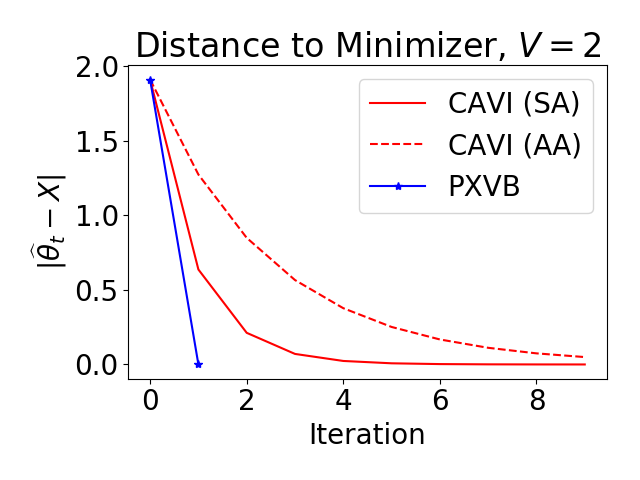
\includegraphics[width=\textwidth]{Probit_real/nm_convergence1.png}
        %\subcaption{}
    \end{subfigure}
          \begin{subfigure}[t]{0.35\textwidth}
        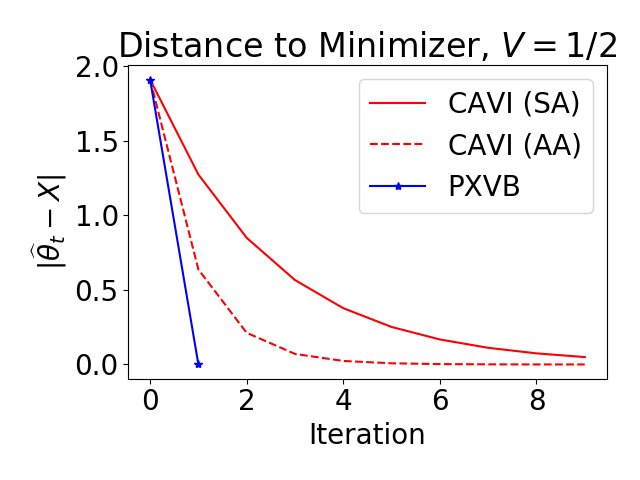
\includegraphics[width=\textwidth]{Probit_real/nm_convergence2.png}
        %\subcaption{}
    \end{subfigure}
    \caption{Convergence results in Normal hierarchical model.}
    \label{nm_case}
\end{figure}


\newpage

\section{Parameter Expanded Variational Bayes}
\label{PXVB}

We describe here the Parameter Expanded Variational Bayes (PX-VB) algorithm proposed in \cite{Qi}. Suppose we have a data model $p(X,\theta)$, where $\theta =  \{\theta_1, ... , \theta_K\}$ are parameters, and $X$ represents the observed data. In PX-VB, the data model is augmented with an auxiliary parameter $\alpha$. Denote this overparametrized model by $p_\alpha(\theta, X)$; and let $\alpha_0$ be the choice of $\alpha$ where the original model is recovered. PX-VB adds two additional steps to the standard CAVI algorithm. At every iteration, we run one step of CAVI, which outputs an approximate variational distribution. PX-VB then chooses an $\alpha$ with which we will expand the data model. The original objective is then recovered through reparametrization of the variational distribution. In other words, any changes incurred by adjusting the data model from $\alpha_0$ to $\alpha$ is absorbed into the variational distribution $q(\theta)$. 



More precisely, at the $t$-th iteration, PX-VB does the following: 
\begin{enumerate}[(i)]
\item {\bf Coordinate ascent:} Update $q^{(t)}(\theta_i)$, for $i=1:K$ to minimize $D\big( \prod_{i=1}^K q(\theta_i) \| p_{\alpha_0}(\theta, X) \big)$. Let the output of this CAVI step be denoted $\tilde q^{(t)}$. 
\item {\bf Expand:} Choose $\alpha$ to minimize $D\big( \prod_{i=1}^K \tilde q^{(t)}(\theta_i) \| p_\alpha(\theta, X) \big)$.
\item {\bf Reduce:} Choose a reparametrization $\theta \mapsto \hat\theta$ such that
\begin{align*}
D\Big( \prod_{i=1}^K \tilde q^{(t)}(\hat\theta_i) \,\big\|\, p_{0}(\hat\theta, X) \Big) = D\Big( \prod_{i=1}^K \tilde q^{(t)}(\theta_i) \,\big\|\, p_\alpha(\theta, X) \Big)
\end{align*}
Set $q^{(t+1)}(\theta) = \tilde q^{(t)}(\hat\theta)$, and repeat. 
\end{enumerate}


Note that with these two added steps to CAVI, PX-VB remains a descent algorithm. In step 2, our choice of $\alpha$ ensures that the KL decreases, and in step three, we reparametrize $q^{(t)}(x)$ to maintain this KL. Therefore, one iteration of PX-VB should do no worse than one step of CAVI on its own. 

The added steps of PX-VB increase the computational cost compared to CAVI, but with a proper choice of augmentation,  PX-VB often converges in fewer iterations, as we explore in the sequel. We see two explanations for such behavior. Firstly, the reparametrization allows for exploration of the parameter space in directions other than the coordinate axes. In the extreme case of the normal hierarchical model, PX-VB points the trajectory of the updates directly to the correct posterior means. Secondly, running CAVI to find an optimal mean field approximation suffers from slow convergence when the variables in the factorized distribution are strongly correlated. A good reparametrization in PX-VB helps decouple the these variables to achieve faster convergence. 




\section{Example: Probit Regression}
\label{probit}

Following the example in \cite{Qi}, we explore the performance of PX-VB in the setting of Bayesian probit regression. Let $\{t_n\}_{n=1}^N$ be $\{-1,+1\}$--valued random variables. The design matrix $X\in\mathbb R^{N\times D}$ is fixed, and we place a normal prior on the parameter vector $w\in\mathbb R^D$. The generative model is
\begin{align}
w &\sim \mathcal N (0, v_0^2I_{D\times D}) \\
t_n &\sim \text{Bern}(\Phi(w^\mathsf T x_n))\quad n = 1, ..., N \label{eq:gen_probit_1}
\end{align}
where $\Phi$ is the standard normal c.d.f. Equivalently, we can re-write this generative model with latent variables $z_n$ as follows: 
\begin{align}
    w &\sim \mathcal N (0, v_0^2I_{D\times D}) \\
    z_n &\sim \mathcal N (w^\mathsf T x_n, 1)\quad n = 1, ..., N \label{eq:gen_probit_zn}\\
    t_n &= \text{sign}(z_n) \quad n = 1, ..., N \label{eq:gen_probit_2}
\end{align}
A brief computation verifies this equivalence: 
\begin{align}
P(t_n = +1) &= P(z_n \geq 0) \quad \text{(by eqn. \ref{eq:gen_probit_2} )}\\
&= \Phi(w^\mathsf Tx_n) \quad \text{(by eqn. \ref{eq:gen_probit_zn})}
\end{align}
which shows that $t_n$ is Bernoulli with parameter $\Phi(w^\mathsf Tx_n)$. 

\subsection{Parameter updates}
We will work with the second formulation where we introduced the latent $z_n$. To perform mean field variational inference, we take a fully factorized distribution over $\{z_n\}_{n=1}^N$ and $w$. In particular, 
\begin{align}
    q_w(w) &\sim \mathcal N (\hat w, \hat\Sigma_w)\\
    q_{z_n}(z_n) &\sim \mathcal{N}(\hat z_n, 1)\mathbb I\{\text{sign}(z_n) = t_n\} \quad n = 1, ..., N
\end{align}
That is, $q_{z_n}$ follows a truncated normal distribution; $z_n$ is restricted to $[0,\infty)$ or $(-\infty,  0]$ when $t_n=1$ or $t_n=-1$, respectively. Our goal is to find parameters $\{\hat z_n\}_{n=1}^\infty$, $\hat w$, and $\hat\Sigma_w$ to minimize the KL divergence $D\big(q(w) \prod_{n=1}^N q(z_n)\|p(w, z| t)\big)$, where $p(w,z|t)$ is the true posterior distribution. 

Writing out this objective explicitly (see \ref{probit_append}) we find that the coordinate ascent updates for the variational parameters are given by 
\begin{align}
    \hat z_n &= \hat w^T x_n \quad n = 1, ..., N\\
    \Sigma_w &= (X^T X + v_0^{-2} I_{D\times d})^{-1}\\
    \hat w &= (X^T X + v_0^{-2} I_{D\times d})^{-1} XE_q[z]
\end{align}

We seek to use PX-VB to accelerate the convergence of CAVI. Following \cite{Qi}, we augment our model with an auxiliary parameter $\alpha$ as follows: 
\begin{align}
    w &\sim \mathcal N (0, \alpha v_0^2I_{D\times D}) \\
    z_n &\sim \mathcal N (w^\mathsf T x_n, \alpha)\quad n = 1, ..., N \\
    t_n &= \text{sign}(z_n) \quad n = 1, ..., N
\end{align}
In other words, we expanded the original model $p(w,z,t|X)$ to $p_\alpha(w,z,t|X)$ with the relation
\begin{align}
   p_\alpha(w,z,t|X) = p(\alpha w, \alpha z, t|X)
\end{align}

At the $t$th iteration, we run one step of CAVI, resulting in a proposed intermediate approximation denoted $\tilde q^{(t)}$. Then in step (ii) of PX-VB, we minimize $D\big(\tilde q(w) \prod_{n=1}^N \tilde q^{(t)}(z_n) \| p_\alpha(w,z,t|X) \big)$ with respect to $\alpha$ and find the minimizer $\alpha^*$ to satisfy: 
\begin{align}
    \alpha^{*2} = \frac{1}{N+M} \Big(\sum_{n=1}^N E_q[z_n^2] - 2E_q[z_n] \hat w^\mathsf Tx_n + x_n^\mathsf T E_q[w w^\mathsf T] w_n\Big) + \frac{1}{v_0^2(N+M)} E_q[w w^\mathsf T]
\end{align}

And in step (iii) the original model is recovered by taking
\begin{align}
    q^{(t+1)}(w) = \tilde q^{(t)}(w/\alpha^*) \quad \text{and} \quad q^{(t+1)}(z_n) = \tilde q^{(t)}(z_n/\alpha^*)
\end{align}
Note that the added steps in PX-VB are relatively computationally inexpensive, and in the following sections, we explore the gains in the rate of convergence. 

\subsection{Convergence results on simulated data}
We compare the convergence of three algorithms: CAVI, PX-VB, and Newton conjugate gradient trust region. First, we applied these algorithms on simulated data: we took the number of data points to be $N = 500$ and the dimension of the parameter $w$ to be $D= 20$. The results are displayed in figure~\ref{fig:Probit_synth}. 

We see that in comparing CAVI and PX-VB, PX-VB converged in shorter time. The difference in consecutive CAVI iterates reached $10^{-12}$ in about 30 seconds, while PX-VB reached this threshold in about 1/6th the time (figure~\ref{fig:Probit_synth}a). In the ELBO plot (figure~\ref{fig:Probit_synth}b), PX-VB also became close to the optima in two iterations and beat CAVI in wall time. 

The Newton method was the slowest of the three algorithm. In our simulation, an iteration takes $\sim10^2$ more time to compute than a step of CAVI or PXVB. This is due to the high dimensional parameter space, since we have a variational parameter for each of the $N$ data points. 


\begin{figure}[tb]
    \begin{subfigure}[t]{0.49\textwidth}
        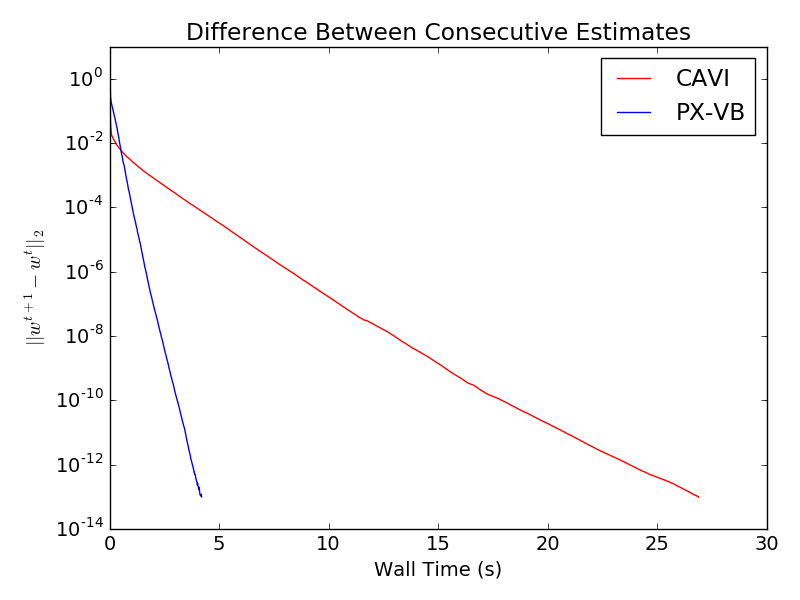
\includegraphics[width=\textwidth]{Probit_synth/CAVI_PX_convergence.png}
        \subcaption{}
    \end{subfigure}
          \begin{subfigure}[t]{0.49\textwidth}
        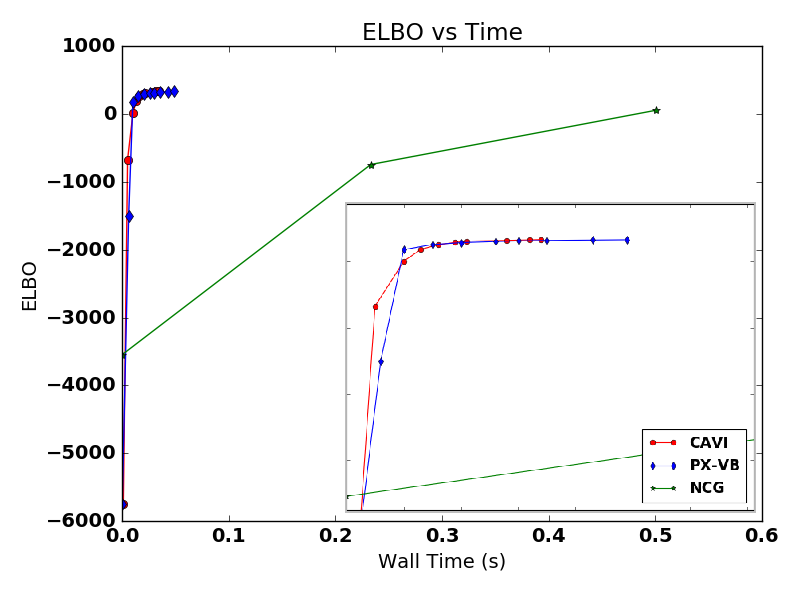
\includegraphics[width=\textwidth]{Probit_synth/elbo_timeII.png}
        \subcaption{}
    \end{subfigure}
    \caption{Convergence results on synthetic data, where $N = 500$ and $D = 20$. (a) The changes in consecutive iterates over time.  (b) The value of our objective function, the evidence lower bound, over time. Inset shows the same plot, zoomed onto the top left quadrant.}
    \label{fig:Probit_synth}
\end{figure}



\subsection{Convergence results on SPAM data}
We also compared the convergence of the three algorithms applied to a probit regression problem on email SPAM data~\cite{Efron}. Here, the observed variables $t_n$ are +1 and -1, indicating whether an email was spam or not spam, respectively. $N=4601$ emails were examined, and each feature vector $x_n$ describes the prevalence of a word or character (such as "money", "free", "!"). In total, there were $57$ features and an added intercept, so $D = 58$. 

Figure~\ref{fig:Probit_spam} shows the rate of convergence of the three algorithms.  Again, Newton is slow compared to CAVI and PX-VB. And PX-VB is exhibits the fastest among all three. 


\begin{figure}[tb]
        \begin{subfigure}[t]{0.49\textwidth}
        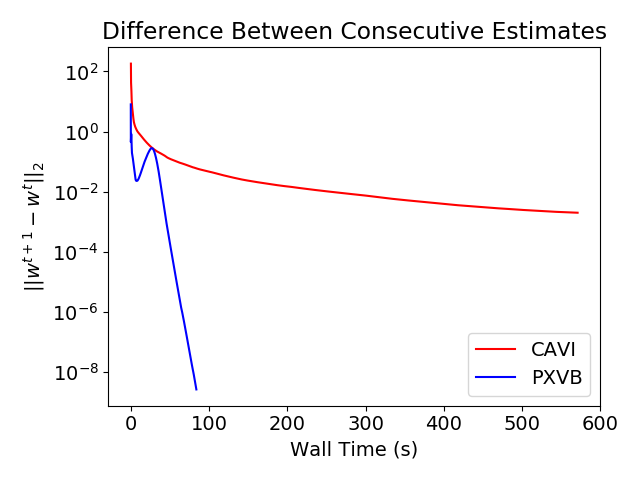
\includegraphics[width=\textwidth]{Probit_real/CAVI_PX_convergence.png}
        \subcaption{}
    \end{subfigure}
          \begin{subfigure}[t]{0.49\textwidth}
        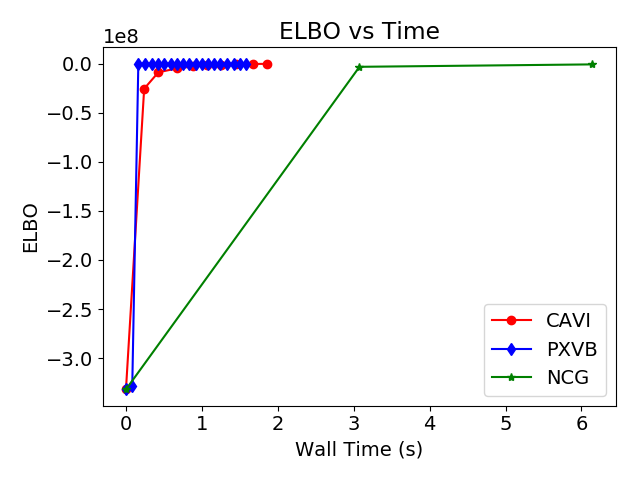
\includegraphics[width=\textwidth]{Probit_real/elbo_time.png}
        \subcaption{}
    \end{subfigure}
    \caption{Convergence results for variational inference on SPAM dataset [2], consisting of $N= 4601$ emails, each with $D=57$ keyword predictors (see examples in table). (a) The differences between consecutive iterates over time. (b) The evidence lower bound over time. } %The consecutive differences in the second order method did not exhibit as much regularity, so they are omitted on the first plot.}
    \label{fig:Probit_spam}
\end{figure}

All three algorithms converged to the same $\hat w$, our variational estimate for the posterior mean for the parameter vector $w$.  Table~\ref{table:Spam_table} shows our estimate for a few selected keywords. Notably, the words "lab", "cs", "meeting", and "george" (the name of the emails' recipient) are strong indicators for an email being not spam, matching our intuition that an email containing work related terms, or knowing the recipient's name, is an indication of not spam. Conversely, emails containingg the \$ or \# are indicative of spam. 


\begin{table}[tb]
%\vspace{2ex}
\begin{tabular}{c | c | c | c | c | c | c | c}
\toprule
\toprule
\textbf{Keyword} & \texttt{intercept} & \texttt{make} & \texttt{3d} & \texttt{addresses} & \texttt{free} & \texttt{business} & \texttt{george} \\
\midrule
Estimate $\widehat w$ & -0.81 & -0.19 & 1.74 & 0.83 & 0.51 & 0.46 & -4.46\\
\midrule
\textbf{Keyword} & \texttt{lab} & \texttt{technology} & \texttt{cs} & \texttt{meeting} & \texttt{!} & \texttt{\$} & \texttt{\#} \\
\midrule
Estimate $\widehat w$ & -7.66 & 0.46 & -1.78 & -1.85 & 0.16 & 2.30 & 1.35\\
\bottomrule
\bottomrule
\end{tabular}
\vspace{0.5em}

\caption{Probit regression analysis of the SPAM dataset. Estimated regression coefficients from CAVI for $14$ example keyword predictors (total number of keywords was 57). Note that the recipient of the emails is named \texttt{george}.}
\label{table:Spam_table}
\end{table}


\section{Example: Linear Mixed Models} 
As in the Probit model, let $X\in \mathbb{R}^{N\times D}$ be a fixed design matrix, with rows $x_n, n = 1,..., N$. We also assume the variances $\sigma^2_\beta, \sigma^2_\mu$, and $\sigma^2_y$ are fixed and known. Let the number of groups be $N_G$, and let the mapping $g(n)\mapsto \{1, ..., N_G\}$ denote the group to which the $n$-th individual belongs. Then the linear mixed model is formulated is follows: 
\begin{align}
\beta &\sim \mathcal N(0, \sigma^2_\beta I_{D\times D}) \label{eq:lmm_prior1}\\
\mu_g &\sim \mathcal N(0, \sigma^2_\mu) \quad \text{for $g= 1, ..., N_G$} \label{eq:lmm_prior2}\\
y_n | \mu_g, \beta &\sim \mathcal N (x_n^T\beta + \mu_{g(n)}, \sigma^2_y)\quad \text{for $n = 1, ..., N$}\label{eq:lmm_LH}
\end{align}
We take a fully factorized distribution over $\beta$ and $\{\mu_g\}_{g=1}^{N_G}$. In particular, 
\begin{align}
q_\beta(\beta) &\sim \mathcal N (\hat \beta, \Sigma_\beta)\\
q_{\mu_g}(\mu_g) &\sim \mathcal{N}(\hat\mu_g, \tau^2_{\mu_g}) \quad \text{for }g = 1, ..., N_G
\end{align}

\subsection{Parameter updates}
The updates for the variational parameters $\hat\beta$, $\Sigma_\beta$, $\hat\mu_g$, and $\tau^2_{\mu_g}$ are standard exponential family computations (see ~\ref{lmm_append}). They are given by 
\begin{align}
{\tau^2_{\mu_g}} &= \Big(\frac{1}{\sigma^2_\mu} + \frac{|\{n : g(n) = g\}|}{\sigma^2_y}\Big)^{-1}\\
{\hat\mu_g} &= \Big(\frac{1}{\sigma^2_\mu} + \frac{|\{n : g(n) = g\}|}{\sigma^2_y}\Big)^{-1}\Big(\frac{1}{\sigma^2_y}\sum_{n: g(n) = g} (y_n - x_n^T\hat\beta)\Big) \label{eq:lmm_mu_upd}
\end{align}
for $g = 1, ..., N_G$. and 
\begin{align}
\Sigma_\beta &= (\frac{1}{\sigma^2_\beta} + \frac{1}{\sigma^2_y}XX^T)^{-1}\\
\hat\beta &= (\frac{1}{\sigma^2_\beta} + \frac{1}{\sigma^2_y}XX^T)^{-1}\Big(\frac{1}{\sigma^2_y}\sum_{n=1}^N  x_n(y_n - \hat\mu_{g(n)} )\Big)
\end{align}

In the parameter expanded model, we keep the priors for $\beta$ and $\mu_g$ the same as in the original model (eqns. \ref{eq:lmm_prior1} \& \ref{eq:lmm_prior2}). The augmentation occurs in the likelihood for $y$, so that
\begin{align}
y_n | \mu_g, \beta &\sim \mathcal N (x_n^T\beta + \mu_{g(n)}+\alpha, \sigma^2_y)\quad \text{for $n = 1, ..., N$} 
\end{align}

The optimal $\alpha$ in step (ii) of PXVB is given by 
\begin{align}
\alpha^* =  \frac{1}{N}\sum_{n=1}^N (y_n - x_n^T\hat\beta - \hat\mu_{g(n)}) \label{eq:lmm_alpha}
\end{align}
And the reparametrization step (iii) is done by 
\begin{align}
    q^{(t+1)}(\mu_g) = \tilde q^{(t)}(\mu_g\alpha^*) \quad \text{and} \quad q^{(t+1)}(\beta) = \tilde q^{(t)}(\beta)
\end{align}
See appendix~\ref{lmm_append} for the derivation of these updates. 



\subsection{Convergence results on simulated data}
We simulated data according the the generative model described in equations \ref{eq:lmm_prior1}-\ref{eq:lmm_LH}. We took $N_G = 10$ groups, and $N/N_G = 50$ observations per group. The dimension of the parameter vector $\beta$ was $D = 20$. The variances $\sigma^2_\beta$ and $\sigma^2_y$ were fixed at 100 and 1, respectively. However, under different settings of $\sigma^2_\mu$, the convergence of PX-VB behaves differently: when $\sigma^2_\mu$ is large, PX-VB exhibits the same behavior as CAVI; but when $\sigma^2_\mu$ is small, PX-VB converges more slowly than CAVI. 

The explanation for the former is straightforward. If we examine the CAVI update for $\hat\mu_g$ (eqn.~\ref{eq:lmm_mu_upd}), then when $\sigma^2_\mu$ is large, it reduces to 
\begin{align}
{\hat\mu_g} &\approx \frac{N_G}{N}\sum_{n: g(n) = g} (y_n - x_n^T\hat\beta) \label{eq:approx_mu}
\end{align}
Now recalling $\alpha^*$ from equation~\ref{eq:lmm_alpha}, we show that this will be close to zero: 
\begin{align}
\alpha &= \frac{1}{N} \sum_{n=1}^N (y_n - x_n^T \hat\beta - \hat\mu_{g(n)})\\
    &= \frac{1}{N} \sum_{g=1}^{N_g} \Big(\sum_{n: g(n)) = g} (y_n - x_n^T \hat\beta)- \frac{N}{N_G}\hat\mu_{g(n)})\Big) \\
    &\approx \frac{1}{N} \sum_{g=1}^{N_g} \Big(\frac{N}{N_g}\hat\mu_g - \frac{N}{N_G}\hat\mu_{g(n)})\Big) \quad \text{(by eqn.~\ref{eq:approx_mu})}\\
    &= 0
\end{align}

Therefore, PX-VB behaves similarly to CAVI when $\sigma_\mu^2$ is large since $\alpha \approx 0$, and our reparametrization step is not doing much. 

When $\sigma_\mu^2$ is small however, our reparametrization appears to hinder the convergence of CAVI. Taking an optimization viewpoint, it is possible that searching in the coordinate direction already corresponds to good directions-- observe CAVI's near linear rate of convergence in figure~\ref{fig:lmm}a, and what appears to be one step convergence of the elbo in figure~\ref{fig:lmm}b-- and therefore, any reparametrization forces the trajectory away from these good directions. 



\begin{figure}[tb]
    \begin{subfigure}[t]{0.49\textwidth}
        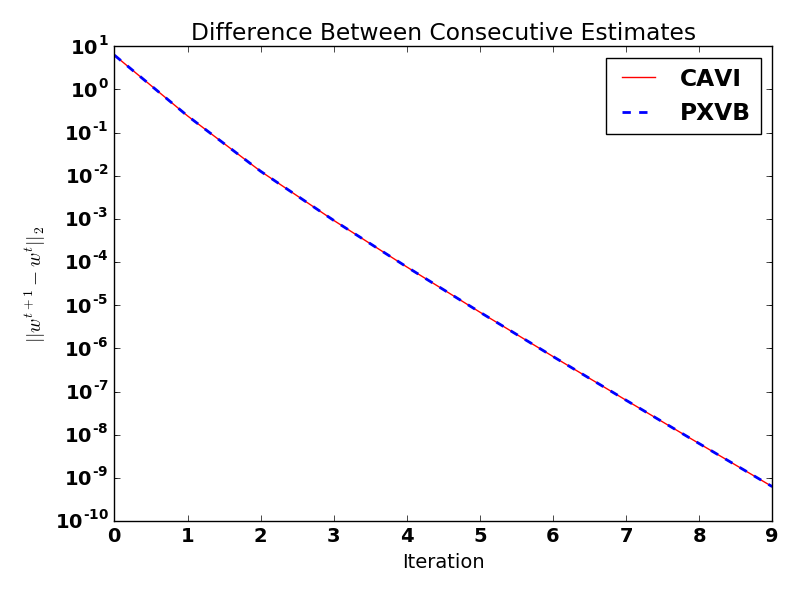
\includegraphics[width=\textwidth]{LMM/pw_lmm_bigvar.png}
        \subcaption{}
    \end{subfigure}
          \begin{subfigure}[t]{0.49\textwidth}
        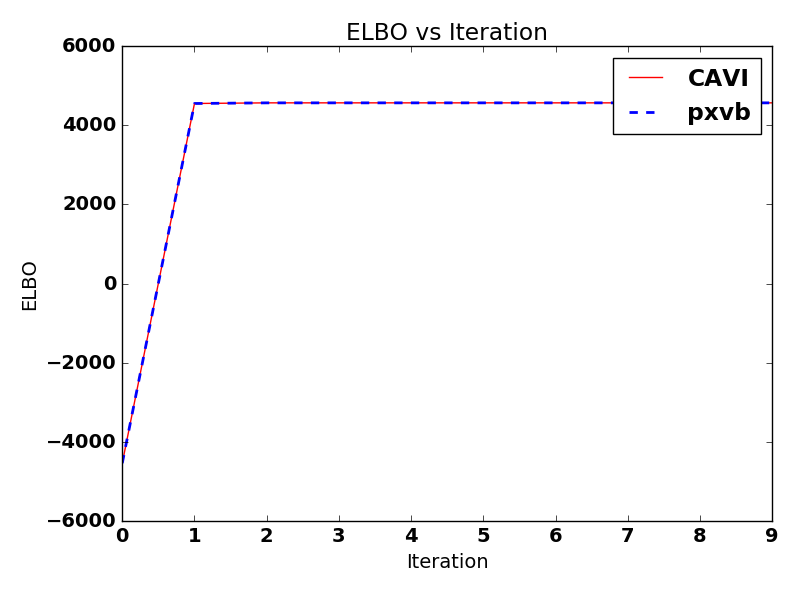
\includegraphics[width=\textwidth]{LMM/elbo_lmm_bigvar.png}
        \subcaption{}
    \end{subfigure}
    \begin{subfigure}[t]{0.49\textwidth}
        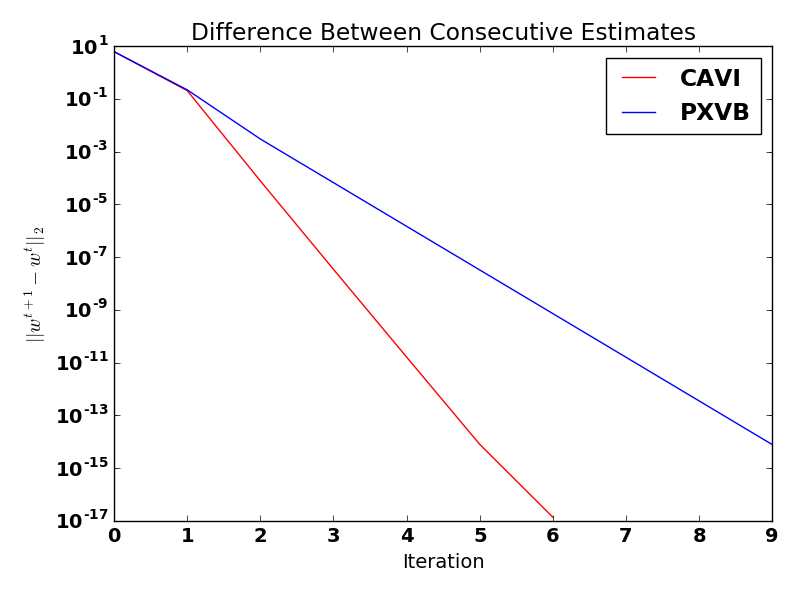
\includegraphics[width=\textwidth]{LMM/pw_lmm_smallvar.png}
        \subcaption{}
    \end{subfigure}
          \begin{subfigure}[t]{0.49\textwidth}
        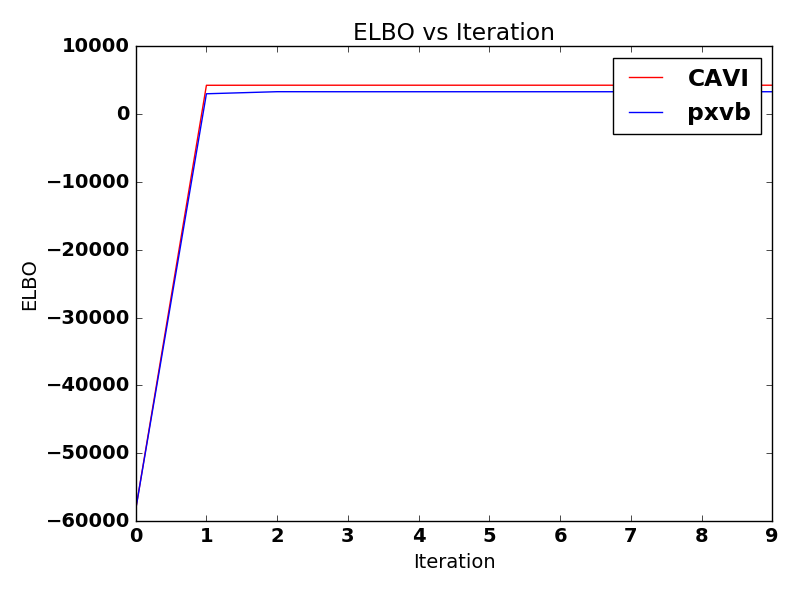
\includegraphics[width=\textwidth]{LMM/elbo_lmm_smallvar.png}
            \subcaption{}
    \end{subfigure}
    \caption{Comparing the convergence of PXVB and CAVI in two regimes. For all plots, there were $N_G = 10$ groups, and $n = 50$ observations per group. The dimension of the parameter vector $\beta$ was $D = 20$. In the {\itshape top row}, the prior variance for $\mu_g$ was $10^{-4}$, while in the {\itshape bottom row}, the prior variance was 100. } %The consecutive differences in the second order method did not exhibit as much regularity, so they are omitted on the first plot.}
    \label{fig:LMM}
\end{figure}




\section{Discussion and future directions}
We found that in our Bayesian probit regression problem, PX-VB speeds up the convergence of variational methods compared to coordinate ascent and Newton conjugate gradient, two standard algorithms in optimization. The advantage to a Newton method is that there exist "black box" implementations of such algorithms in most standard optimization packages. The only requirement is that one must be able to write down the objective function, in our case the evidence lower bound. However, in variational methods, the optimization is often conducted over a high dimensional parameter space. For example, in probit regression, there is one variational parameter for each data point. This results in high computational complexity at each iteration. This phenomenon is well exhibited in our results, where Newton suffers in terms of wall time, even though the number of iterations required for convergence is smaller than CAVI or PX-VB. 

Thus, this result suggest that there are real gains in convergence time to deriving updates for coordinate descent. While CAVI requires more iterations to converge than Newton, each iteration is very cheap to compute. 

PX-VB introduces an intermediate step to coordinate ascent, but the computational cost of this additional step is often small---and with a good augmentation, this additional computational cost is made worthwhile by the gains in per-iteration rate of convergence as demonstrated in the Probit model.

To see this more abstractly, we can view the intermediate step in PX-VB as defining a mapping $M$ that takes $(q, p_0) \stackrel{\text{(ii)}}{\mapsto} (q, p_\alpha) \stackrel{\text{(iii)}}{\mapsto} (q_\alpha, p_0)$. Moreover, let $S$ be the mapping defined by the CAVI updates, and assume that the truth $q^*$ is a fixed point of both the mappping $S$ and $M$. Then the error of each iteration of PX-VB can be seen as
\begin{align}
\|q^{(t+1)} - q^*\|_2 &\leq \| M(S(q^{(t)})) - q^*\|_2 \\
&\leq \|MS\|_2 \|q^{(t)} - q^*\|_2\\
&\leq \|M\|_2\|S\|_2 \|q^{(t)} - q^*\|_2
\end{align}

Thus, we see that while CAVI converges linearly at rate $\|S\|_2$, PX-VB converges at rate $\|M\|_2\|S\|_2$. Whenever the largest eigenvalue of $M$ is less than $1$, PX-VB will converge faster than CAVI. 

It is possible that our choice of reparametrization in the linear mixed model did not fall into this regime. Therefore, one challenge to PX-VB is anticipating which data-augmentation scheme will actually accelerate convergence. 

{\color{red} 

It is well known that the mean field approximation performs well when the posterior distribution has low correlation. Therefore, we would like to understand the connection between the reparametrization mapping $M$ and the posterior correlation structure. ~\\~\\

Ultimately, in the normal hierarchical model, data augmentation methods correspond to choosing good directions for coordinate ascent. We would like to look at more examples where PX-VB succeeds and understand whether, more generally, these directions make use of second-order structure.
}

\newpage

\section*{Acknowledgments}
We would like to thank Professor Wainwright and Fanny for their dedication to teaching an excellent course! We also thank Ryan Giordano in the Department of Statistics, for introducing us to the ASIS paper \cite{Yu} and for his helpful discussions.

% also thank ryan %Also thanks to the stat department lounge for housing us since we got here.

\section*{Attribution}
\begin{itemize}
\item Runjing Liu: 
\item Jake Soloff: 
\end{itemize}

\begin{thebibliography}{10}

\bibitem{Barber} Barber, D. (2012). Bayesian Reasoning and Machine Learning. {\sl Cambridge University Press}.

\bibitem{Beal} Beal, M. (2003). Variational Algorithms for Approximate Bayesian Inference. {\sl Doctoral dissertation}, Gatsby Computational Neuroscience Unit, University College London.

\bibitem{Blei} Blei, D. M., Kucukelbir, A. \& McAuliffe, J. D. (2016). Variational Inference: a Review for Statisticians. {\itshape arXiv:1601.00670}.

\bibitem{Cooper} Cooper, G.F. (1990). The Computational Complexity of Probabilistic Inference using Bayesian Belief Networks. {\sl Artificial Intelligence.} 42(2), 393–405.

\bibitem{Efron} Efron, B \& Hastie, T.J. (2016). Computer Age Statistical Inference. {\itshape Cambridge University Press}.

\bibitem{Grimmer} Grimmer, J. (2011). An Introduction to Bayesian Inference via Variational Approximations. {\itshape Political Analysis}. 19(1): 32-47.

\bibitem{Luo} Luo, Z. Q. \& Tseng, P. (1992). On the Convergence of the Coordinate Descent Method for Convex Differentiable Minimization. {\itshape Journal of Optimization Theory and Applications} 72(1): 7-35. 

\bibitem{Papaspiliopoulos} Papaspiliopoulos, O., Roberts, G. O., and Skold, M. (2003), Non-Centered Parameterisations for Hierarchical Models and Data Augmentation. {\sl Bayesian Statistics} 307-326

\bibitem{Qi} Qi, Y. \& Jaakkola, T. S. (2006). Parameter Expanded Variational Bayesian Methods. {\itshape Neural Information Processing Systems}. 

\bibitem{Sahu} Sahu, S. K., \& Roberts, G. O. (1998). On Convergence of the EM Algorithm and the Gibbs Sampler. {\sl Statistics
and Computing}. 

\bibitem{van} van Dyk, D. A., \& Meng, X. L. (2001). The art of data augmentation (with discussion). {\sl Journal of Computational and Graphical Statistics}.

\bibitem{Yu} Yu, Y. \& Meng, X. (2012). To Center or Not to Center: That Is Not the
Question-- An Ancillarity-Sufficiency Interweaving Strategy (ASIS) for Boosting MCMC Efficiency. {\itshape Journal of Computational and Graphical Statistics}. 20(3): 531-570. 
\end{thebibliography}

\newpage

\appendix

\section{Proofs of Propositions}

\begin{proof} (of {\bf Proposition 1}) From \cite{Barber} [ch. 8] we know the conditionals have the form 
\begin{align}
p(\theta_1\mid X,\theta_2) 
%&= \mathcal N(\theta_1; \mu_1^*+\Sigma_{12}\Sigma_{22}^{-1}(\theta_2-\mu_2^*),\Sigma_{11} - \Sigma_{12}\Sigma_{22}^{-1}\Sigma_{21}), \\
&= \mathcal N(\theta_1; \mu_1^*-\Lambda_{22}^{-1}\Lambda_{21}(\theta_2-\mu_2^*),\Lambda_{22}^{-1}), \\
p(\theta_2\mid X,\theta_1) 
%&= \mathcal N(\theta_2; \mu_2^*+\Sigma_{21}\Sigma_{11}^{-1}(\theta_1-\mu_1^*),\Sigma_{22} - \Sigma_{21}\Sigma_{11}^{-1}\Sigma_{12}).
&= \mathcal N(\theta_2; \mu_2^*-\Lambda_{11}^{-1}\Lambda_{12}(\theta_1-\mu_1^*),\Lambda_{11}^{-1}).
\end{align}
Let $\widehat\theta = (\widehat\theta_1,\widehat\theta_2)$. The conditionals give the form of the CAVI variational factors \cite{Blei}
\begin{align}
q^{(t+1)}(\theta_1) &= 
\mathcal N(\theta_1; \underbrace{\mu_1^*-\Lambda_{22}^{-1}\Lambda_{21}(\widehat\theta_2^{(t)}-\mu_2^*)}_{=\widehat\theta_1^{(t+1)}},\Lambda_{22}^{-1}), \\
q^{(t+1)}(y) 
&= \mathcal N(\theta_2; \underbrace{\mu_2^*-\Lambda_{11}^{-1}\Lambda_{12}(\widehat\theta_1^{(t)}-\mu_1^*)}_{=\widehat\theta_2^{(t+1)}},\Lambda_{11}^{-1}).
\end{align}
This gives the update for each variational mean. Rewriting these updates,
\begin{align}
\widehat\theta_1^{(t+1)} - \mu_1^*  
&= -\Lambda_{22}^{-1}\Lambda_{21}(\widehat\theta_2^{(t)}-\mu_2^*)
=\Lambda_{22}^{-1}\Lambda_{21}\Lambda_{11}^{-1}\Lambda_{12}(\widehat\theta_1^{(t)}-\mu_1^*) \\
\widehat\theta_2^{(t+1)} - \mu_2^*  
&= -\Lambda_{11}^{-1}\Lambda_{12}(\widehat\theta_1^{(t)}-\mu_1^*)
=\Lambda_{11}^{-1}\Lambda_{12}\Lambda_{22}^{-1}\Lambda_{21}(\widehat\theta_2^{(t)}-\mu_2^*)
\end{align}
Note that if $\lambda$ is an eigenvalue of one of these matrices, say $\Lambda_{22}^{-1}\Lambda_{21}\Lambda_{11}^{-1}\Lambda_{12} v = \lambda v$, then 
$$
\Lambda_{11}^{-1}\Lambda_{12}\Lambda_{22}^{-1}\Lambda_{21}(\Lambda_{11}^{-1}\Lambda_{12} v) = \lambda (\Lambda_{11}^{-1}\Lambda_{12}v)
$$
\noindent and similarly in the other direction, so the spectra of these matrices coincide. Let $\gamma = \|\Lambda_{22}^{-1}\Lambda_{21}\Lambda_{11}^{-1}\Lambda_{12}\|_2 = \|\Lambda_{11}^{-1}\Lambda_{12}\Lambda_{22}^{-1}\Lambda_{21}\|_2$, so the rate of convergence of each variational mean is
\begin{align}
\left\|\widehat\theta_i^{(t+1)} - \mu_i^*\right\|_2
&\le \gamma\left\|\widehat\theta_i^{(t)} - \mu_i^*\right\|_2,
\end{align}
for $i=1,2$. Hence the rate of convergence for the whole algorithm is $\gamma$, since
\begin{align}
\left\|(\widehat\theta_1^{(t+1)},\widehat\theta_2^{(t+1)})-(\mu_1^*,\mu_2^*)\right\|_2^2
&=\left\|\widehat\theta_1^{(t+1)}-\mu_1^*\right\|_2^2 + \left\|\widehat\theta_2^{(t+1)}-\mu_2^*\right\|_2^2\\
&\le \gamma^2\left\|\widehat\theta_1^{(t)}-\mu_1^*\right\|_2^2 + \gamma^2\left\|\widehat\theta_2^{(t)}-\mu_2^*\right\|_2^2 \\
&= \gamma^2\left\|(\widehat\theta_1^{(t)},\widehat\theta_2^{(t)})-(\mu_1^*,\mu_2^*)\right\|_2^2 
\end{align}
This rate $\gamma$ matches the rate of convergence of the corresponding block Gibbs sampler \cite{Sahu}.
\end{proof}


\begin{proof} (of {\bf Proposition 2}) $\|S(T(x))-S(T(y))\|_2\le \gamma_S\|T(x) - T(y)\|_2 \le \gamma_S\gamma_T\|x-y\|_2$.%, proving the claim. %We also note some consequences of this basic observation relevant to our work. Define $x^{2k+1} = S(x^{2k})$ and $x^{2k+2} = T(x^{2k+1})$ for $k\ge 0$. Then the iterates $\{x^k\}$ converge linearly with rate at most $\sqrt{\gamma_S\gamma_T}$. Also, even if one of the operators, say $S$, is non-expansive, their composition $S\circ T$ is a contraction, so the alternating iterates will have a fixed point. 
\end{proof}


\newpage


\section{Probit Model Calculations}
\label{vi}

\noindent{\bf Computing the ELBO.} Recall that the ELBO is given by:
\begin{align}
\mathcal L &= E_q[\log p(w,t,z|X)] + H(q) \\
	&=  E_q[\log p(w)] + \Big(\sum_{n=1}^N E_q[\log p(z_n,t_n|w,X)]\Big) - \Big(\sum_{i=1}^n E_q[\log q(z_n)]\Big) - E_q[\log q(w)] 
\end{align} 
We examine each of these terms individually. First, 
\begin{align}
E_q[\log p(w)] &= -\frac{1}{2v_0^2} E_q[w^Tw] + K
	= -\frac{1}{2v_0^2} (\text{Tr}(\Sigma_w) + \hat w^T \hat w) + K
\end{align}

where $K$ is some constant in each line independent of the variational parameters. Now we recall some facts about truncated Gaussians. If $z_n\sim \mathcal N(\hat z_n, 1)$, and lies on the interval $[0,\infty)$ when $t_n=1$ or on the interval $(-\infty, 0]$ when $t_n=-1$, then 
\begin{align}
Ez_n = \hat z_n + t_n\frac{\phi(-\hat z_n)}{\Phi(t_n\hat z_n)}
\text{ and }
Ez_n^2 = 1 + \hat z_n^2 + t_n\hat z_n \frac{\phi(-\hat z_n)}{\Phi(t_n\hat z_n)}
\end{align}
where $\phi$ and $\Phi$ are the normal p.d.f and normal c.d.f., respectively. Hence, %if $t_n = 1$, then 
\begin{align}
E_q[\log p(z_n,t_n|w,X)] 
%&= -\frac{1}{2}E_q[(z_n - w^Tx_n)^2]  + K \\
	%&=  -\frac{1}{2} E_q[z_n^2] + \hat w^Tx_n E_q[z_n] - \frac{1}{2} x_n^T E[ww^T]x_n + K \\
	&= 
	-\frac{1}{2}\Big(1 + \hat z_n^2  + t_n\hat z_n \frac{\phi(-\hat z_n)}{\Phi(t_n\hat z_n)}\Big) 
	+ \hat w^Tx_n\Big(\hat z_n +t_n \frac{\phi(-\hat z_n)}{\Phi(t_n\hat z_n)}\Big) \\
	&~~~~~- \frac{1}{2} \Big(x_n^T(\Sigma_w + \hat w \hat w^T)x_n\Big) + K 
\end{align}
%and if $t_n = -1$ then 
%\begin{align}
%E_q[\log p(z_n,t_n|w,X)] 
%	&=  -\frac{1}{2} E_q[z_n^2] + \hat w^T x_n E_q[z_n] - \frac{1}{2} x_n^T E[ww^T]x_n + K \\
%	&= -\frac{1}{2}\Big(1 + \hat z_n^2 - \hat z_n \frac{\phi(-\hat z_n)}{\Phi(-\hat z_n)}\Big)
%	 + \hat w^T x_n\Big(\hat z_n - \frac{\phi(-\hat z_n)}{\Phi(-\hat z_n)}\Big)  
%	  - \frac{1}{2} \Big(x_n^T(\Sigma_w + \hat w \hat w^T)x_n\Big)+ K 
%\end{align}
And the entropy for $z_n$ conditional on $t_n$ is given by %restricted to $[0,\infty)$ is given by 
\begin{align}
H[q(z_n)] &= - E_q[\log q(z_n)] 
	= \log\Big(\sqrt{2\pi e} \Phi(t_n\hat z_n)\Big) - \frac{1}{2}t_n\hat z_n\frac{ \phi(-\hat z_n)}{\Phi(t_n\hat z_n)}
\end{align}
Finally, we compute the entropy of $q(w)$, a normal distribution: 
\begin{align}
H(q(w)) &= -E_q[\log q(w) ] = \frac{1}{2}\log \big((2\pi e)^D |\Sigma_w|)
\end{align}

%And therefore, we conclude that
%\begin{align}
%\sum_{n=1}^N &E_q[\log p(z_n,t_n|w,X)] + E_q[\log q(z_n) \\
%	&= \sum_{n=1}^N\Bigg(  \mathbb I\{t_n = 1\}\log\Big(\sqrt{2\pi e} (1- \Phi(-%\hat z))\Big) + \mathbb I\{t_n = 0\}\log\Big(\sqrt{2\pi e} \Phi(-\hat z)\Big) + \frac{1}{2}(\hat z)^2\Bigg)
%\end{align}


%\begin{align}
%\log p(w,t,z|X) &= \log p(w) + \sum_{n=1}^N \log p(z_n,t_n|w,X) \\
%	&= -\frac{1}{2v_0} w^Tw + \sum_{n=1}^N -\frac{1}{2}(-z_n - \hat z)^2 %\mathbb I\{t_n = \text{sign}(z_n)\}
%\end{align}

Putting together the pieces, the ELBO is given by
\begin{align*}
\mathcal L = 
%- \frac{1}{2v_0^2}& (\text{Tr}(\Sigma_w) + \hat w^T \hat w) 
%+  \frac{1}{2}\log \big((2\pi e)^D |\Sigma_w|)\\
%&+\sum_{n : t_n = 1} -\frac{1}{2}\Big(1 + \hat z_n^2  + \hat z_n \frac{\phi(-\hat z_n)}{1 - \Phi(-\hat z_n)}\Big) + \hat w^Tx_n\Big(\hat z_n + \frac{\phi(-\hat z_n)}{1 - \Phi(-\hat z_n)}\Big) + \log\Big(\sqrt{2\pi e} (1- \Phi(-\hat z_n))\Big) - \frac{1}{2}\hat z_n\frac{ \phi(-\hat z_n)}{1 - \Phi(-\hat z_n)}\\
%&+\sum_{n : t_n = -1} -\frac{1}{2}\Big(1 + \hat z_n^2 - \hat z_n \frac{\phi(-\hat z_n)}{\Phi(-\hat z_n)}\Big)
%	 + \hat w^T x_n\Big(\hat z_n - \frac{\phi(-\hat z_n)}{\Phi(-\hat z_n)}\Big)  
%	  +\log\Big(\sqrt{2\pi e} \Phi(-\hat z_n)\Big) + \frac{1}{2}\hat z_n\frac{ \phi(-\hat z_n)}{\Phi(-\hat z_n)}\\
%&+ \sum_{n=1}^N - \frac{1}{2} \Big(x_n^T(\Sigma_w + \hat w \hat w^T)x_n\Big)\\
%- \frac{1}{2v_0^2}& (\text{Tr}(\Sigma_w) + \hat w^T \hat w) 
%+  \frac{1}{2}\log \big((2\pi e)^D |\Sigma_w|) 
%+ \sum_{n=1}^N - \frac{1}{2} \Big(x_n^T(\Sigma_w + \hat w \hat w^T)x_n\Big) \\
%&+\sum_{n=1}^N
% -\frac{1}{2}\Big(1 + \hat z_n^2  + t_n\hat z_n \frac{\phi(-\hat z_n)}{\Phi(t_n\hat z_n)}\Big) 
% + \hat w^Tx_n\Big(\hat z_n + t_n\frac{\phi(-\hat z_n)}{\Phi(t_n\hat z_n)}\Big) 
% + \log\Big(\sqrt{2\pi e} (\Phi(t_n\hat z_n))\Big) 
% - \frac{1}{2}t_n\hat z_n\frac{ \phi(-\hat z_n)}{\Phi(t_n\hat z_n)}\\
= - \frac{1}{2v_0^2}& (\text{Tr}(\Sigma_w) + \hat w^T \hat w) 
+  \frac{1}{2}\log \big((2\pi e)^D |\Sigma_w|) 
+ \sum_{n=1}^N - \frac{1}{2} \Big(x_n^T(\Sigma_w + \hat w \hat w^T)x_n\Big) \\
&+\sum_{n=1}^N
 -\frac{1}{2}\Big(1 + \hat z_n^2  + 2t_n(\hat z_n-\hat w^Tx_n) \frac{\phi(-\hat z_n)}{\Phi(t_n\hat z_n)}\Big) 
 + \hat w^Tx_n\hat z_n 
 + \log\Big(\sqrt{2\pi e} (\Phi(t_n\hat z_n))\Big) 
\end{align*}



\noindent{\bf CAVI Updates.} 
%The simplest approach to variational inference maximizes the ELBO $\cl$ via coordinate-ascent, i.e. choosing the best value of a variational parameter with all others fixed. Iteratively applying these updates, the variational approximation $q$ improves at every step toward some local optimum. Conditional conjugacy yields closed form updates for $\widehat\gamma_k$ and $\widehat\lambda_{kl}$:

\begin{itemize}
\item {\bf Update to } 
\item {\bf Update to }
\end{itemize}

\noindent{\bf PX-VB Updates.} 

\newpage

\section{Linear Mixed Model Calculations}
\noindent{\bf Computing the ELBO}: 
We compute the ELBO
\begin{align}
\mathcal L &= E_q[\log p(y,\mu,\beta|X)] + H(q) \\
	&=-\frac{1}{2\sigma^2_\beta}E_q[\beta^T\beta] - \frac{1}{2\sigma^2_\mu}\sum_{g=1}^{N_G} E_q[\mu_g^2] - \frac{1}{2\sigma^2_y}\sum_{n=1}^N E_q[(y_n - x_n^T\beta - \mu_{g(n)})^2] -\sum_{g=1}^{N_g}E_q[\log q_{\mu_g}] - E_q[\log q_\beta(\beta)]
\end{align} 

We examine each of these terms individually. First, 
\begin{align}
-\frac{1}{2\sigma^2_\beta} E_q[\beta^T\beta] = -\frac{1}{2\sigma^2_\beta} (\text{Tr}(\Sigma_\beta) + \hat \beta^T \hat\beta) 
\end{align}

Next, 
\begin{align*}
- \frac{1}{2\sigma^2_\mu}\sum_{g=1}^{N_G} E_q[\mu_g^2] = - \frac{1}{2\sigma^2_\mu}\sum_{g=1}^{N_G}(\tau^2_{\mu_g} + \hat\mu_g^2)
\end{align*}

Furthermore, 
\begin{align*}
 - \frac{1}{2\sigma^2_y}\sum_{n=1}^N &E_q[(y_n - x_n^T\beta - \mu_{g(n)})^2] \\
 &=  - \frac{1}{2\sigma^2_y}\sum_{n=1}^N \Big(E_q[\mu_{g(n)}^2] - 2\hat\mu_{g(n)}(y_n - x_n^T\hat\beta) + E_q[(x_n^T\beta)^2] - 2y_n (x_n^T\hat\beta)\Big)\\
 &= - \frac{1}{2\sigma^2_y}\sum_{n=1}^N \Big((\tau^2_{\mu_{g(n)}} + \hat\mu_{g(n)}^2) - 2\hat\mu_{g(n)}(y_n - x_n^T\hat\beta)\Big) - \frac{1}{2\sigma^2_y} \text{Tr}(X^T(\Sigma_\beta + \hat\beta\hat\beta^T)X) + \frac{1}{\sigma^2_y} y^TX^T\hat\beta
\end{align*}
And the entropy of a Gaussian is given by 
\begin{align*}
-E_q[\log q_{\mu_g}(\mu_g)] = \frac{1}{2} \log(2\pi e \sigma_{\mu_g}^2)\\
-E_q[\log q_{\beta}(\beta)] = \frac{1}{2} \log((2\pi e)^D |\Sigma_{\beta}|)
\end{align*}

Putting the pieces together, 
\begin{align*}
\mathcal L = -\frac{1}{2\sigma^2_\beta} (\text{Tr}(\Sigma_\beta) + \hat \beta^T \hat\beta)- &\frac{1}{2\sigma^2_\mu}\sum_{g=1}^{N_G}(\tau^2_{\mu_g} + \hat\mu_g^2)- \frac{1}{2\sigma^2_y}\sum_{n=1}^N \Big((\tau^2_{\mu_{g(n)}} + \hat\mu_{g(n)}^2) - 2\hat\mu_{g(n)}(y_n - x_n^T\hat\beta)\Big) - \frac{1}{2\sigma^2_y} \text{Tr}(X^T(\Sigma_\beta + \hat\beta\hat\beta^T)X) \\
&+ \frac{1}{\sigma^2_y} y^TX^T\hat\beta+\sum_{g=1}^{N_G}\frac{1}{2} \log(2\pi e \tau_{\mu_g}^2) + \frac{1}{2} \log((2\pi e)^D |\Sigma_{\beta}|)
\end{align*}
 
\noindent{\bf CAVI updates}
We examine the log likelihood, and derive our updates by exploiting the fact that our likelihood and variational distributions are exponential families. Firstly, 
\begin{align*}
\log p(y, \mu, \beta | X) = -\frac{1}{2\sigma^2_\beta}\beta^T\beta - \frac{1}{2\sigma^2_\mu}\sum_{g=1}^{N_G} \mu_g^2 - \frac{1}{2\sigma^2_y}\sum_{n=1}^N (y_n - x_n^T\beta - \mu_{g(n)})^2 + K
\end{align*}
For a choice $g\in\{1, ..., N_G\}$, we seek the updates for $\mu_g$. We take expectations of the log likelihood with respect to the variational distribution of $\beta$ and $\mu_i$ $i\not=g$, dropping constants independent of $\mu_g$: 
\begin{align*}
E_{\beta, \mu_{(-g)}} [ \log p(y, \mu, \beta | X) ] &=  - \frac{1}{2\sigma^2_\mu} \mu_g^2 - \frac{1}{2\sigma^2_y}\sum_{n: g(n) = g} E_{\beta}[(y_n - x_n^T\beta - \mu_{g})^2] + K\\
	&= - \frac{1}{2\sigma^2_\mu} \mu_g^2 - \frac{|\{n : g(n) = g\}|}{2\sigma^2_y} \mu_g^2 + \frac{\mu_g}{\sigma^2_y}\sum_{n: g(n) = g} (y_n - x_n^T\hat\beta) + K
\end{align*}
Now recall that the canonical parametrization of a Gaussian in exponential family form is given by $\log p(x) = -\frac{1}{2\sigma^2} x^2 + \frac{\mu}{\sigma^2}x + K$. Comparing these two forms, the updates for $\mu_g$ must satisfy
\begin{align*}
\frac{1}{\tau^2_{\mu_g}} &= \frac{1}{\sigma^2_\mu} + \frac{|\{n : g(n) = g\}|}{\sigma^2_y}\\
\frac{\hat\mu_g}{\tau^2_{\mu_g}} &= \frac{1}{\sigma^2_y}\sum_{n: g(n) = g} (y_n - x_n^T\hat\beta)
\end{align*}
Rearranging, 
\begin{align*}
{\tau^2_{\mu_g}} &= \Big(\frac{1}{\sigma^2_\mu} + \frac{|\{n : g(n) = g\}|}{\sigma^2_y}\Big)^{-1}\\
{\hat\mu_g} &= \Big(\frac{1}{\sigma^2_\mu} + \frac{|\{n : g(n) = g\}|}{\sigma^2_y}\Big)^{-1}\Big(\frac{1}{\sigma^2_y}\sum_{n: g(n) = g} (y_n - x_n^T\hat\beta)\Big)
\end{align*}
We use a similar technique to find the updates for $\beta$. Taking expectations with respect to all the $\mu_g$'s, 
\begin{align*}
E_\mu[\log p(y, \mu, \beta | X) ] &=  -\frac{1}{2\sigma^2_\beta}\beta^T\beta  - \frac{1}{2\sigma^2_y}\sum_{n=1}^N ((x_n^T\beta)^2 - 2(x_n^T\beta)(y_n - \hat\mu_{g(n)} )) + K\\
	&=  -\frac{1}{2\sigma^2_\beta}\beta^T\beta  - \frac{1}{2\sigma^2_y} \beta^TXX^T\beta + \frac{1}{\sigma^2_y}\beta^T\Big(\sum_{n=1}^N  x_n(y_n - \hat\mu_{g(n)} )\Big) + K
\end{align*}
And comparing with the canonical exponential family paramatrization, we conclude that the updates are given by
\begin{align*}
\Sigma_\beta &= (\frac{1}{\sigma^2_\beta} + \frac{1}{\sigma^2_y}XX^T)^{-1}\\
\hat\beta &= (\frac{1}{\sigma^2_\beta} + \frac{1}{\sigma^2_y}XX^T)^{-1}\Big(\frac{1}{\sigma^2_y}\sum_{n=1}^N  x_n(y_n - \hat\mu_{g(n)} )\Big)
\end{align*}


\noindent{\bf PX-VB updates}
In step (ii) of PX-VB, we minimize $D\big( \prod_{i=1}^K q(\theta_i) \| p_{\alpha}(\theta, X) \big)$. Writing out this KL divergence, 
\begin{align}
E_q\Big[ \log \frac{p_\alpha(y|\mu, \beta) p(\mu)p(\beta)}{q(\mu)q(\beta)}\Big] &= E_q\Big[\log p_\alpha(y|\mu, \beta)\Big] + K
\end{align}
where we absorbed terms independent of $\alpha$ into $K$. Therefore, we seek to minimize $E_q\Big[\log p_\alpha(y|\mu, \beta)\Big]$ with respect to $\alpha$. Continuing, 
\begin{align}
E_q\Big[\log p_\alpha(y|\mu, \beta)\Big] = \sum_{n=1}^N (y - x_n^T\beta - \mu_{g(n)} - \alpha)^2
\end{align}
Taking a derivative of the above, setting it equal to 0, we find $\alpha^*$ must satisfy 
\begin{align}
\alpha^* = \frac{1}{N}
\sum_{n=1}^N (y - x_n^T\beta - \mu_{g(n)})  
\end{align}

In the reparametrization step (iii), we seek a reparametrization $\mu\mapsto \hat\mu$ and $\beta\mapsto \hat\beta$ such that $p_\alpha(y | \mu, \beta) = p_0(y | \hat\mu,\hat\beta)$. Explictly, we seek 
\begin{align}
y_n - x_n^T \beta - \mu_{g(n)} - \alpha = y_n - x_n^T \hat\beta - \hat\mu_{g(n)} 
\end{align}
So we reparametrize by setting $\hat\beta = \beta$ and $\hat\mu_g = \mu_g - \alpha$. 

\newpage

\section{Normal Means Model Calculations}
\label{normal}

\noindent{\bf Sufficient Augmentation.} Returning to the sufficient augmentation version of the normal-normal model above, 
\begin{align}
q(\mu)
&\triangleq \cn(\widehat\mu,\widehat\sigma_\mu^2) \\
q(\theta)
&\triangleq \cn(\widehat\theta_S,\widehat\sigma_{\theta_S}^2)
\end{align}
We are optimizing the variational parameters, denoted by $\text{hat}\widehat{\text{s}}\,$. Writing out the ELBO
\begin{align}
\cl(q)
&=\EE_{q}\bigg[\log \frac{p(X,\mu,\theta)}{q(\mu)q(\theta)}\bigg] 
=  \EE_{q}\bigg[\log p(X\mid \mu)\bigg]
-  \EE_{q}\bigg[\log\frac{q(\mu)}{p(\mu\mid \theta)} \bigg]
-  \EE_{q}\bigg[\log \frac{q(\theta)}{p(\theta)}\bigg] \\
&=  \frac{2X\widehat\mu -  \widehat\sigma_{\mu}^{2} - \widehat\mu^{2}}{2} %\EE_q\bigg[-(x-\mu)^2\bigg]
+\log\widehat\sigma_\mu - \frac{\widehat\sigma_\mu^{2}+\widehat\sigma_{\theta_S}^{2} + (\widehat\mu-\widehat\theta)^2}{2V}
+\log \widehat{\sigma}_{\theta_S} 
%\EE_q\bigg[\log \frac{q(\theta)}{p(\theta)}\bigg] 
+ \text{const.}
\end{align}

\noindent {\bf Ancillary Augmentation.} For the ancillary augmentation, let
\begin{align}
\widetilde q(\nu)
&\triangleq \cn(\widehat{\nu},\widehat\sigma_\nu^2) \\
\widetilde q(\theta)
&\triangleq \cn(\widehat\theta_A,\widehat\sigma_{\theta_A}^2).
\end{align}
Again writing out the ELBO,
\begin{align}
\cl(\widetilde q)
&=\EE_{\widetilde q}\bigg[\log \frac{p(X,\nu,\theta)}{\widetilde q(\nu)\widetilde q(\theta)}\bigg] 
=  \EE_{\widetilde q}\bigg[\log p(X\mid \nu,\theta)\bigg]
-  \EE_{\widetilde q}\bigg[\log\frac{\widetilde q(\nu)}{p(\nu)} \bigg]
-  \EE_{\widetilde q}\bigg[\log \frac{\widetilde q(\theta)}{p(\theta)}\bigg] \\
&=  \frac{2X\widehat\nu+2X\widehat\theta - 2\widehat\nu\widehat\theta - \widehat\sigma_\nu^2-\widehat\nu^2-\widehat\sigma_{\theta_A}^2-\widehat\theta^2}{2}
+\log\widehat\sigma_\nu - \frac{\widehat\sigma_\nu^{2} + \widehat\nu^2}{2V}
+\log \widehat{\sigma}_{\theta_A} 
%\EE_q\bigg[\log \frac{q(\theta)}{p(\theta)}\bigg] 
+ \text{const.}
\end{align}
The coordinate ascent updates are
\begin{align}
\widehat\nu^{(t+1)}
&= \frac{V(X - \widehat\theta^{(t)})}{1+V} \\%\frac{X + V\widehat\theta^{(t)}}{1+V} \\
\widehat\sigma^{2(t+1)}_{\nu}
&= \frac{V}{1+V} \\
\widehat\theta^{(t+1)}
&= X-\widehat\nu^{(t+1)} \\
\widehat\sigma^{2(t+1)}_{\theta_A}
&= 1
\end{align}
The variational parameter for the posterior mean of $\theta$ given $X$ satisfies
\begin{align}
\left|\widehat\theta^{(t+1)} - X\right|
&= \left|\widehat\nu^{(t+1)}\right| 
= \frac{V}{1+V}\left|X - \widehat\theta^{(t)}\right|,
\end{align}
this parameter converges geometrically with rate $\frac{V}{1+V}$. \\






\end{document}